%!TEX root = ../main.tex
\section{Der minimalistische Comp}
Es gibt eine große Anzahl an Webseiten, bei denen die Seiten mit unnötigen Elementen oder Werbung überladen sind. Als Grundidee hat dieser Design-Entwurf daher, dass die Seite minimalistisch gehalten wird, um damit soviel wie möglich auszudrücken bei gleichzeitig minimalem Design.  
Diese Seite ist entsprechend dem Responsive Design Principle\footcite[vgl.][]{alistapart:rwd} auch für Handhelds und Tablets geeignet.
	\subsection{Comprehensive Dummy}
Der zeichnerische Entwurf (siehe Abbildung \ref{mini_comp1}) zeigt, wie die Grundidee umgesetzt werden soll. Im Anschluss wurde dieser in HTML und CSS implementiert.

\begin{figure} [hp]
	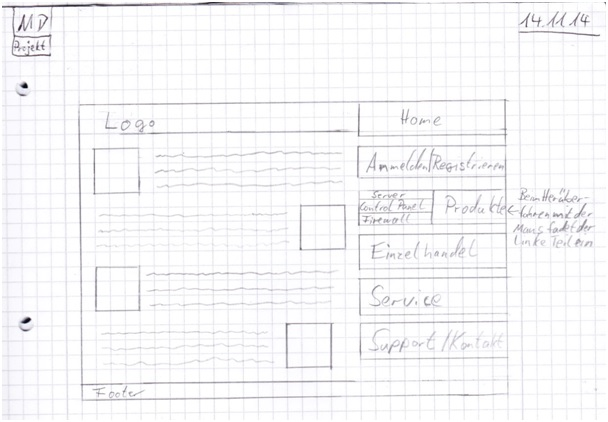
\includegraphics[width=\textwidth]{./img/mini_comp1.png}
	\caption{Die Umsetzung der Idee auf Papier}
	\label{mini_comp1}
\end{figure}

	\subsection{Entwicklungsphase HTML\&CSS}
Der erste Entwurf des Comps wurde in HTML umgesetzt. Einzig und allein das Mark-Up reicht jedoch nicht aus um die Struktur des Entwurfs darzustellen, wie es im finalen Comprehensive Dummy der Fall ist. (siehe Abbildung \ref{mini_comp2})

\begin{figure} [hp]
	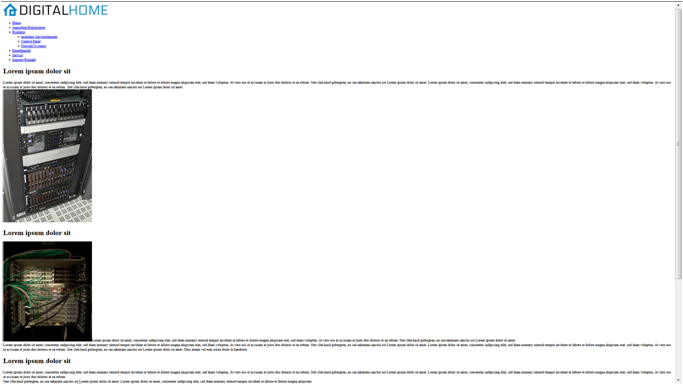
\includegraphics[width=\textwidth]{./img/mini_comp2.png}
	\caption{Die erste Umsetzung in HTML}
	\label{mini_comp2}
\end{figure}

Durch die Implementation von CSS-Klassen nimmt das Design entsprechend des Entwurfs allmählich Form an. Hierbei bereitete die Menüleiste Probleme, da anfangs noch manche Elemente aus dem Footer, Content und Header überdeckt sind. Da Unterkategorien direkt bei den Navigationspunkten in der vorgesehenen Anordnung nicht funktioniert haben, wurde dies letztendlich herausgenommen. Die Unterpunkte werden stattdessen dann angezeigt, wenn auf den jeweiligen Navigationspunkt geklickt wird. Ein Fehler, bei dem andere Elemente von der Navigationsleiste überdeckt wurden, ist durch Anpassen der Breiten und Höhen der Elemente beseitigt.
Das Responsive Design bereitete anfangs ebenfalls Probleme. Nach einigem Aufwand und trotz dem Verzicht auf etwaige Unterkategorien konnte der Entwurf der Zeichnung ähnlich konstruiert werden. (siehe Abbildung \ref{mini_comp3})

\begin{figure} [hp]
	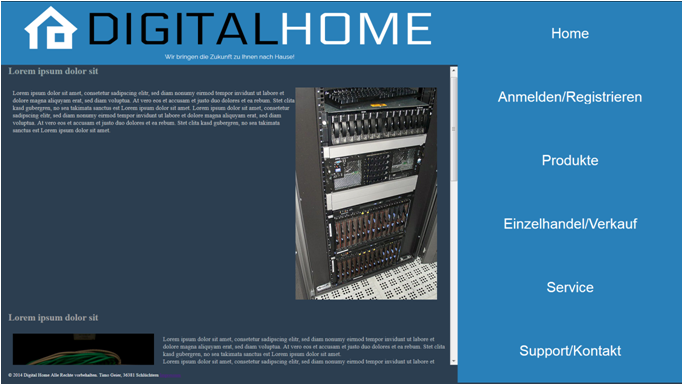
\includegraphics[width=\textwidth]{./img/mini_comp3.png}
	\caption{Die endgültige Umsetzung in HTML und CSS}
	\label{mini_comp3}
\end{figure}

	\subsection{Farbgebung}
	\label{farb_mini}

Da der Webshop Digitale Haustechnik verkauft, sollten die Farben offen und sehr intelligent wirken, zudem eine gewisse Ruhe und Kühle ausstrahlen. Aber es sollte auch zum Minimalismus des Seitenaufbaus passen.
Deswegen basiert das Farbschema in der Online-Fassung hauptsächlich auf blauen Farbtönen, wie in der Abbildung \ref{mini_farb1} zu sehen ist. Die Hintergrundfarbe und die Footerfarbe sind in einem dunklen Blau gehalten, das Ruhe, Konzentration und Sachlichkeit symbolisiert. 
Sowohl der Header, als auch die Elemente der Navigationsleiste sind in unterschiedlichen Blautönen, je nachdem, ob mit dem Cursor über den Header oder die Elemente der Navigationsleiste gefahren wird. Sie sollen offen und intelligent wirken. Zusätzlich sind diese Farben im Kontrast zum Hintergrund und Footer, wodurch sie sehr im Fokus stehen.
Die Überschriften und die Texte sind in jeweils zwei unterschiedlichen Grautönen gefärbt. Diese sollen die Sachlichkeit, Funktionalität, Schlichtheit, und den Minimalismus der Seite vermitteln. Zudem können die Absätze dadurch besser voneinander unterschieden werden.
Die Schriftfarbe des Footers ist weiß, um die Lesbarkeit zu erhöhen. Er enthält wichtige Informationen über das Copyright, den Webseitenbetreiber und zudem einen Link zum Impressum der Seite. 
	\begin{figure} [hp]
	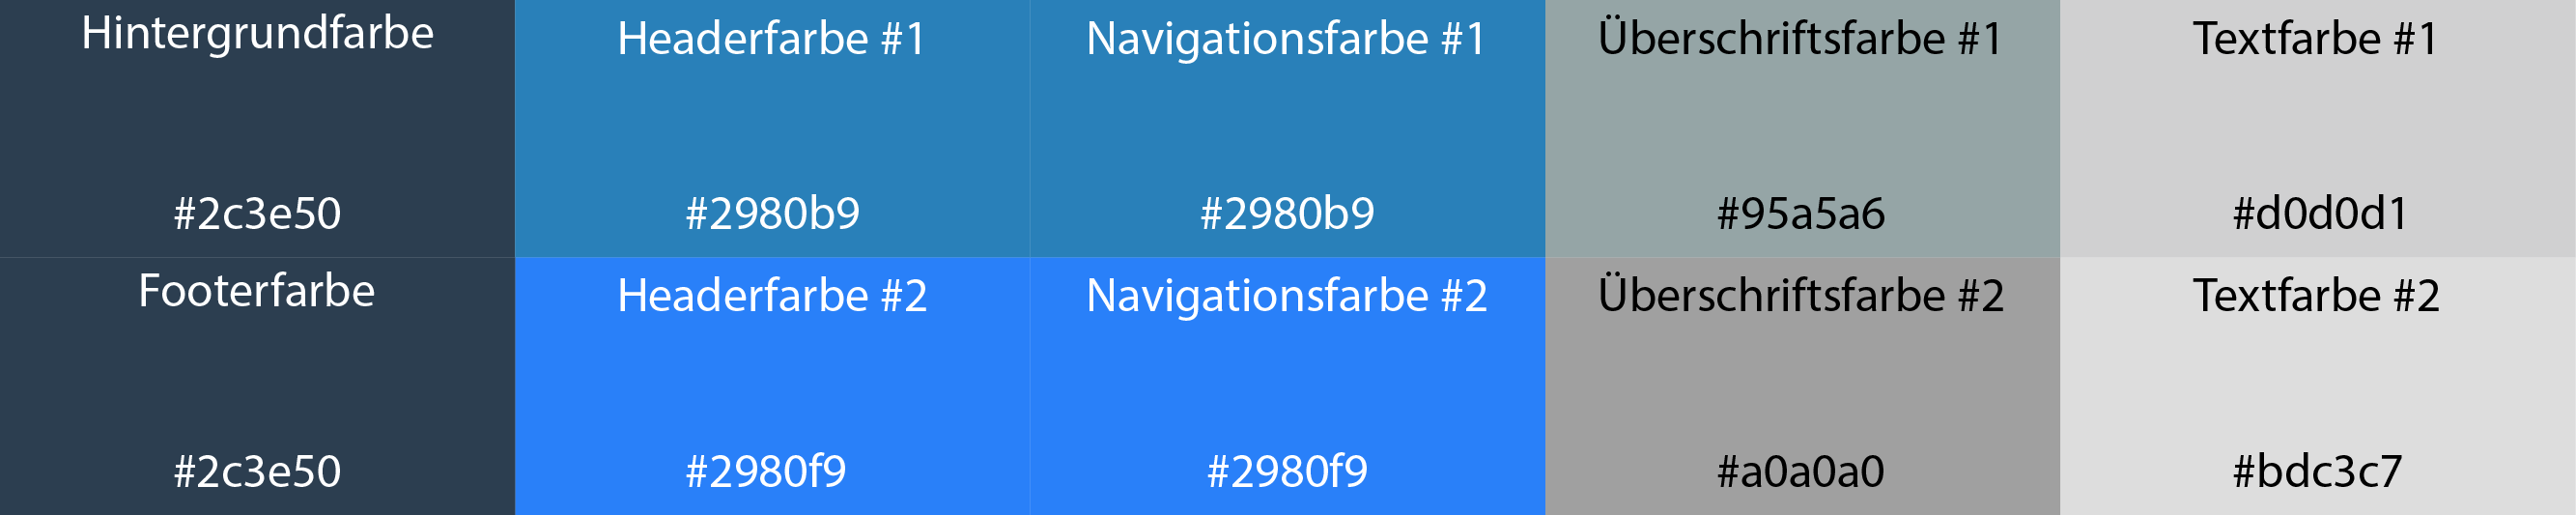
\includegraphics[width=\textwidth]{./img/mini_farb1.png}
	\caption{Das Hauptfarbschema}
	\label{mini_farb1}
\end{figure}

Als 1. alternatives Farbschema wurde ein geteilt komplementäres Farbschema gewählt. Dieses steht sehr im Kontrast zum Hauptfarbschema. (siehe Abbildung \ref{mini_farb2}) 
Die Hintergrundfarbe ist orange mit einem Gelbstich. Die ist positiv besetzt, und symbolisiert zudem Sonnenschein und Kreativität. Dadurch wirkt die ganze Webseite auch ungezwungener, was bei der Vermarktung von Produkten auch wichtig ist. Zusätzlich vermittelt orange eine gute Wohnatmosphäre.
Für den Header und die Navigationsleiste wird die Komplementärfarbe zu orange, blau, verwendet. Diese steht für Offenheit, Intelligenz und Vertrautheit. Dadurch passt es auch zu dem Angebot der digitalen Haustechnik. 
Der Text ist in schwarz beziehungsweise dunklen Grautönen gehalten, und ist somit ein guter Kontrast zum Hintergrund. Zusätzlich drückt sie Eleganz und Stärke aus.

\begin{figure} [hp]
	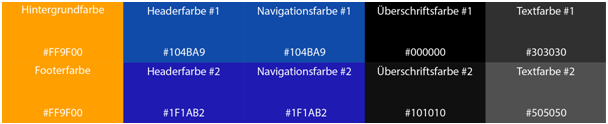
\includegraphics[width=\textwidth]{./img/mini_farb2.png}
	\caption{Das 1. alternative Farbschema }
	\label{mini_farb2}
\end{figure}

Als 2. alternatives Farbschema wurde ein komplementäres Farbschema gewählt. Dieses steht wieder sehr im Kontrast zum Hauptfarbschema. (siehe Abbildung \ref{mini_farb3})
Die Hintergrundfarbe ist ein kräftiges Orange, was auch Kreativität und Sonne und dadurch auch Wärme symbolisiert. Zusätzlich ist sie positiv besetzt und drückt auch eine gemütliche Atmosphäre aus.
Der Header und die Navigationsleiste sind in der Komplementärfarbe von orange, türkisblau,  gefärbt. Diese wirkt sehr lebendig und hat einen hohen Kontrast zum Hintergrund.
Der Text ist in Grautönen, wodurch die Lesbarkeit des Inhalts gewährleistet wird. Zudem unterstreicht es den Minimalismus des Webseitenlayouts.

\begin{figure} [hp]
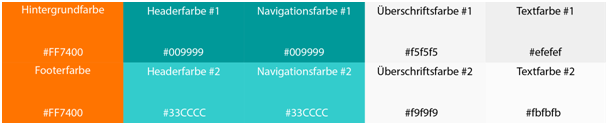
\includegraphics[width=\textwidth]{./img/mini_farb3.png}
\caption{Das 3. alternative Farbschema }
\label{mini_farb3}
\end{figure}

	\subsection{Typographische Gestaltung}\label{chapter:mini:typo}

Als Schriftart wurde die Schriftart „Raleway“ gewählt, da sie sehr innovativ und technisch wirkt. Diese unterstreicht das Minimalistische im Design. (für weitere Begründung vgl. Kapitel \ref{typo_inno} und Kapitel \ref{typo_zeit})
Die Schriftgrößen sind möglichst groß gewählt, um den Inhalt der Seite sehr besser lesbar zu gestalten.
Die Schriftfarben sind so gewählt, das diese einen guten Kontrast zum Hintergrund bieten, und dadurch nochmals die Lesbarkeit erhöhen. (siehe Kapitel \ref{farb_mini})


	\subsection{Strukturanalyse der Seite}
Wie in Abbildung \ref{mini_comp3} zu sehen, beinhaltet der Header das Logo mit einem Werbespruch.
Die Navigation sitzt auf der rechten Seite, da diese Seite sich aus der Masse hervorheben soll, denn viele Seiten haben standardmäßig auf der linken Seite oder oben unterhalb des Headers ihre Navigationsleiste. Diese soll ein Drittel des Platzes auf der Webseite einnehmen, damit diese trotzdem sehr schnell zur Geltung kommt. Zudem wird hierdurch der goldene Schnitt im Design verwendet, was bekannter maßen für viele Menschen eine besondere ästhetik verleiht.
Der Content soll zwischen Header und Footer sein, und wird horizontal von der Navigationsleiste eingeschränkt. Dabei soll er bei Textseiten so strukturiert sein, dass bei jedem Abschnitt ein Bild abwechselnd auf der linken und auf der rechten Seite hat. Somit wirkt es trotz des minimalistischen Designs nicht zu eintönig. Auf Seiten mit vielen Bildern, zum Beispiel der Seite mit der Produktübersicht, sollen die Elemente tabellarisch und dem Responsive Design Principle entsprechend dynamisch angeordnet sein.
Der Footer enthält Informationen über das Copyright, dem Webseiten-Betreiber sowie ein Link zum Impressum.
